\chapter{Five Online Businesses and the Discipline of Choosing}

This chapter follows a School of Hard Knocks entrepreneurship interview curated by LazyingArt LLC through Video2Book. The speaker is not giving a mathematical blackboard lecture; he is sorting five online business models by practical fit, income path, and operating constraint. We will keep that rhythm. First comes the selection rule, then the five models: creator work, video editing, e-commerce, social media marketing, and online courses.

\section{Choosing by Endurance, Not Hype}

The opening move is important. The speaker begins by saying that he is not there to sell anything. He is sharing the online businesses he personally likes for 2022. That matters because the list is not a promise of automatic income. It is a menu of work.

The first principle is not ``choose the hottest model.'' It is closer to an endurance test. If every route requires daily effort before it becomes useful, then the first question is what kind of work we can keep doing.

\begin{equation}
N_{\mathrm{models}} = 5.
\end{equation}

The five models are not ranked by ease. They are introduced as possible directions:

\begin{equation}
\mathcal{B}
=
\{\text{creator work},\ \text{video editing},\ \text{e-commerce},\ \text{social media marketing},\ \text{online courses}\}.
\end{equation}

A compact way to express the speaker's selection rule is this:

\begin{equation}
\text{fit}
\approx
\text{interest}
+
\text{willingness to repeat the work}.
\end{equation}

This is not a formula for guaranteed success. It is a discipline for choosing. The business that looks attractive from the outside may not survive contact with the daily routine. The business that fits one's curiosity has a better chance of surviving the slow accumulation of skill.

\begin{figure}
\centering
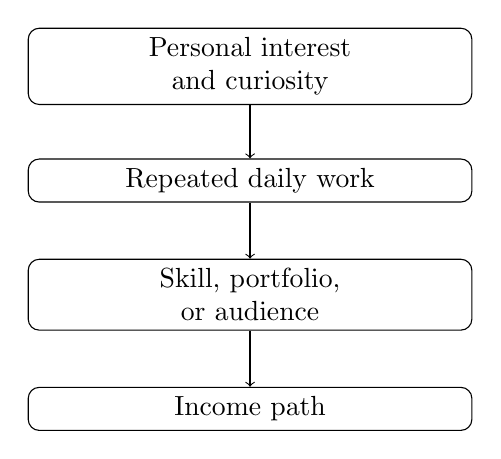
\begin{tikzpicture}[x=1cm,y=1cm]
\node[draw, rounded corners, align=center, text width=5.4cm] (interest) at (0,0) {Personal interest\\and curiosity};
\node[draw, rounded corners, align=center, text width=5.4cm] (repeat) at (0,-1.45) {Repeated daily work};
\node[draw, rounded corners, align=center, text width=5.4cm] (skill) at (0,-2.9) {Skill, portfolio,\\or audience};
\node[draw, rounded corners, align=center, text width=5.4cm] (income) at (0,-4.35) {Income path};
\draw[->] (interest) -- (repeat);
\draw[->] (repeat) -- (skill);
\draw[->] (skill) -- (income);
\end{tikzpicture}
\caption{The lecture's opening filter: interest matters because it sustains the repetition needed to build skill, audience, or portfolio.}
\end{figure}

\section{Creator Work: Audience as an Asset}

The first business model is being a creator. The speaker immediately divides it into two routes. One route is building a personal brand around oneself: vlogs, gaming, business content, or another recognizable niche. The other route is creating content for a brand.

\begin{equation}
\text{creator work}
=
\text{personal brand}
\quad \text{or} \quad
\text{content for brands}.
\end{equation}

The personal-brand route is attractive because it can create several income paths from the same audience. The speaker names ad revenue from platforms such as TikTok and YouTube, brand deals, and later businesses built on the trust of the audience. Once people are invested in who the creator is and what the creator is doing, that attention can support other projects, such as a skincare company or a clothing line.

The brand-deal range is given as an example, not as a guaranteed rate:

\begin{equation}
D_{\mathrm{brand\ deal}}
\approx
\$500 \text{ to } \$5{,}000
\quad \text{per promotion}.
\end{equation}

The mechanism is straightforward. Attention creates distribution; distribution creates options.

\begin{align}
\text{personal brand}
&\longrightarrow
\text{audience},\\
\text{audience}
&\longrightarrow
\{\text{ad revenue},\ \text{brand deals},\ \text{new businesses}\}.
\end{align}

The second creator route is service work for other companies. Businesses need daily social content: user-generated content, reviews, product explanations, and event announcements. The speaker mentions JT Barnett as an example of someone working in the space of connecting creators with companies, so that creators can become faces for new brands.

\subsection{Question \& Answer}

\paragraph{Question.}
What if we want to build a personal brand, but the personal brand cannot yet support us full time?

\paragraph{Answer.}
The lecture's answer is to separate the long-term asset from the near-term service. We can build the personal brand in the background while creating content for other brands as paid work. In symbols, the bridge looks like this:

\begin{align}
\text{early creator}
&=
\text{personal brand under construction}
+
\text{brand content services},\\
\text{brand content services}
&\longrightarrow
\text{cash flow while the audience grows}.
\end{align}

This is a useful distinction. The personal brand is an owned asset, but the service work can make the craft economically survivable before that asset is large enough.

\section{Video Editing: Selling Time Back to Creators}

The second business model moves behind the camera. Video editing is for people who like the content creation space but do not necessarily want to appear on camera. The speaker adds a practical qualification: the editor should have a good eye for what makes content interesting, which usually means consuming content regularly enough to understand its rhythms.

The demand argument is a time argument. Companies are moving more heavily into digital space, and creators do not always have time to break down their content for every platform. A YouTube vlogger may need clips for TikTok, Instagram, and a YouTube clips channel. That repackaging is work.

Let \(T_c\) be the creator's available time and \(T_r\) the time required to repurpose content across platforms. The opportunity appears when

\begin{equation}
T_r > \text{time the creator wants to spend on repurposing}.
\end{equation}

Then the editor sells saved time:

\begin{equation}
\text{editor value}
\approx
\text{saved creator time}
+
\text{platform-ready output}.
\end{equation}

\paragraph{A worked entry path.}
The lecture gives a simple sequence for getting started.

\begin{enumerate}
\item Learn the craft from online resources: YouTube, Google, Udemy, Skillshare, and strong working editors.
\item Study examples of effective editing; the speaker names Hillier Smith, who edited for Logan Paul.
\item Offer services on platforms such as Fiverr and Upwork.
\item Use early jobs to earn practice, build a portfolio, and prepare to approach larger creators or brands.
\end{enumerate}

We can write this as an update rule for the beginner's position:

\begin{equation}
\text{portfolio}_{n+1}
=
\text{portfolio}_{n}
+
\text{completed client work}_{n}.
\end{equation}

The point is not that marketplaces are the final destination. The point is that they can supply the first observable evidence that the editor can deliver.

\section{E-Commerce: Scale With Operational Demands}

The third business model shifts from media labor into product ownership. E-commerce is attractive when someone makes a product, wants to sell a specific item, or wants to start a clothing brand online. The speaker likes the scalability: a good brand can become larger than the founder and, in the optimistic case, something that can be passed on.

But this section changes tone quickly. E-commerce is described as one of the harder models because it asks for business judgment. It is not enough to sell at launch. A brand has to acquire customers again and again.

A minimal way to express the constraint is:

\begin{equation}
\text{sustainable e-commerce}
\neq
\text{launch customers only}.
\end{equation}

The business must keep solving customer acquisition:

\begin{equation}
\text{customer demand}_{\mathrm{year}}
=
\text{launch demand}
+
\sum_{m=2}^{12}\text{monthly acquisition}_{m}.
\end{equation}

There is also a capital requirement. The speaker names two uses of capital: ordering products and marketing them.

\begin{equation}
C_{\mathrm{startup}}
=
C_{\mathrm{product}}
+
C_{\mathrm{marketing}}.
\end{equation}

The advice is still encouraging, but it is not careless. If someone is passionate about clothing or a brand idea, the speaker says to research, study other websites and brands, model what works, and go all in. The mechanism is imitation plus execution, not passive inspiration.

\section{Social Media Marketing: Local Businesses and Monthly Retainers}

The fourth model returns to service work, but now the client is a local business. The speaker uses a restaurant. The restaurant may already have good food and good customer service, but it may not be showing its food, menu, and events online.

This is the problem statement:

\begin{equation}
\text{good product/service}
+
\text{weak online visibility}
\longrightarrow
\text{marketing opportunity}.
\end{equation}

The proposed service is monthly management. The marketer approaches the owner, explains the visibility gap, agrees on a fee, then manages the social media month by month. The speaker gives an example range:

\begin{equation}
R_{\mathrm{monthly}}
\approx
\$500 \text{ to } \$1{,}500
\quad \text{per month}.
\end{equation}

The work includes taking pictures of food and menus, learning about upcoming events, and posting that material. But the speaker adds a sharper point: to separate oneself from weaker competitors, it is worth learning ads on Facebook, Instagram, and other platforms.

\subsection{Question \& Answer}

\paragraph{Question.}
If the business already has good food, good products, and good service, what problem are we actually solving?

\paragraph{Answer.}
We are not solving the product problem. We are solving the visibility and reach problem. If the business starts with little or no following, posting alone may produce zero engagement and zero views. In that case, the client is spending money without getting a return.

A simple decision rule is:

\begin{equation}
\text{if organic reach} \approx 0,
\qquad
\text{then posting alone is not the solution}.
\end{equation}

The service becomes more complete when it includes the ability to create reach:

\begin{align}
\text{monthly management}
&=
\text{content}
+
\text{posting}
+
\text{platform knowledge},\\
\text{stronger offer}
&=
\text{monthly management}
+
\text{advertising ability}.
\end{align}

\begin{figure}
\centering
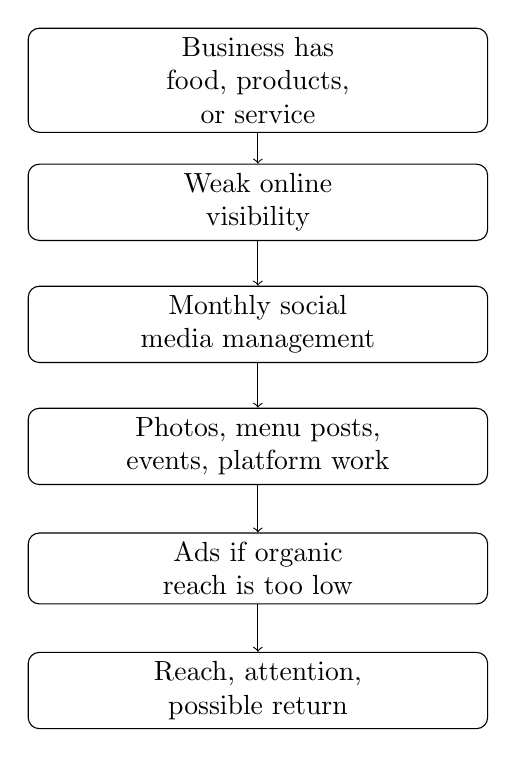
\begin{tikzpicture}[x=1cm,y=1cm]
\node[draw, rounded corners, align=center, text width=5.6cm] (product) at (0,0) {Business has\\food, products,\\or service};
\node[draw, rounded corners, align=center, text width=5.6cm] (visibility) at (0,-1.55) {Weak online\\visibility};
\node[draw, rounded corners, align=center, text width=5.6cm] (retainer) at (0,-3.1) {Monthly social\\media management};
\node[draw, rounded corners, align=center, text width=5.6cm] (content) at (0,-4.65) {Photos, menu posts,\\events, platform work};
\node[draw, rounded corners, align=center, text width=5.6cm] (ads) at (0,-6.2) {Ads if organic\\reach is too low};
\node[draw, rounded corners, align=center, text width=5.6cm] (return) at (0,-7.75) {Reach, attention,\\possible return};
\draw[->] (product) -- (visibility);
\draw[->] (visibility) -- (retainer);
\draw[->] (retainer) -- (content);
\draw[->] (content) -- (ads);
\draw[->] (ads) -- (return);
\end{tikzpicture}
\caption{The restaurant example: the service begins with visibility, but the deeper problem is reach and return.}
\end{figure}

\section{Online Courses: Packaging Expertise for Reach}

The fifth model is creating an online course. This is for someone who is already expert at something or successful in a field and can teach others a process. The transcript is slightly garbled here, but the clear meaning is that the course should give students an A-to-Z framework for following the teacher's path in their own way.

The speaker's example is a custom shoe design business. A course could explain materials, how to get started, how to work on different shoes, and the practical process behind the business.

The structure is:

\begin{align}
\text{expertise}
&\longrightarrow
\text{framework},\\
\text{framework}
&\longrightarrow
\text{course},\\
\text{course}
&\longrightarrow
\text{additional income stream}.
\end{align}

The speaker is careful about scale here. He frames the course more as a side hustle or additional income stream than as the main business. The distribution problem is solved partly through marketplaces: Udemy and Skillshare allow the course to reach people beyond the creator's existing followers and personal network.

\begin{equation}
\text{course reach}
=
\text{existing audience}
+
\text{marketplace audience}.
\end{equation}

The entrepreneurial lesson is the same as before: an asset becomes more valuable when it has a channel. Expertise by itself is private. A course turns it into a product. A marketplace gives that product more surface area.

\section{Compact Model Comparison}

We can summarize the lecture as five ways of converting a different asset into income. This is a reconstruction from the transcript, not a board diagram.

\begin{figure}
\centering
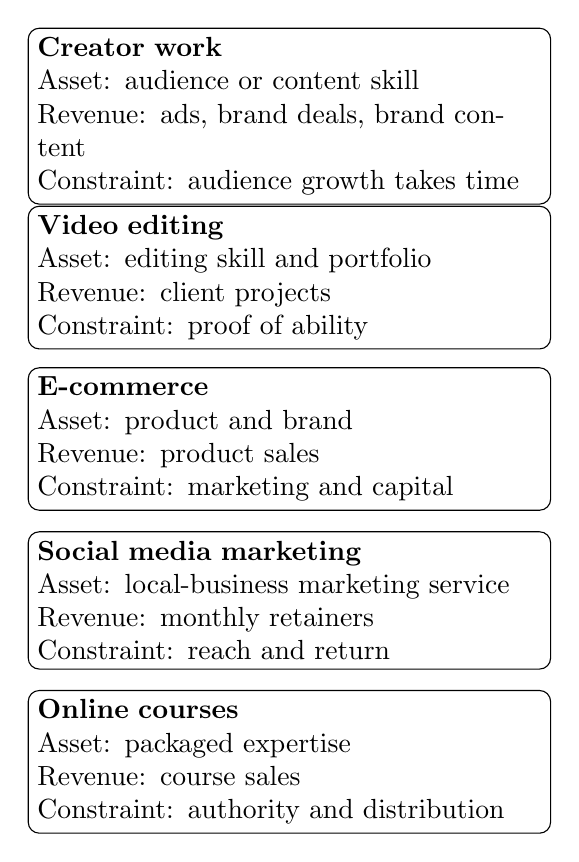
\begin{tikzpicture}[x=1cm,y=1cm]
\node[draw, rounded corners, align=left, text width=6.4cm] at (0,0)
{\textbf{Creator work}\\
Asset: audience or content skill\\
Revenue: ads, brand deals, brand content\\
Constraint: audience growth takes time};

\node[draw, rounded corners, align=left, text width=6.4cm] at (0,-2.05)
{\textbf{Video editing}\\
Asset: editing skill and portfolio\\
Revenue: client projects\\
Constraint: proof of ability};

\node[draw, rounded corners, align=left, text width=6.4cm] at (0,-4.1)
{\textbf{E-commerce}\\
Asset: product and brand\\
Revenue: product sales\\
Constraint: marketing and capital};

\node[draw, rounded corners, align=left, text width=6.4cm] at (0,-6.15)
{\textbf{Social media marketing}\\
Asset: local-business marketing service\\
Revenue: monthly retainers\\
Constraint: reach and return};

\node[draw, rounded corners, align=left, text width=6.4cm] at (0,-8.2)
{\textbf{Online courses}\\
Asset: packaged expertise\\
Revenue: course sales\\
Constraint: authority and distribution};
\end{tikzpicture}
\caption{The five models differ less by being ``online'' than by the asset each one asks us to build.}
\end{figure}

\section{Summary}

The lecture is a list, but the useful structure underneath the list is a set of tradeoffs. Creator work builds audience; video editing sells time back to creators; e-commerce builds a product brand; social media marketing sells visibility and reach to existing businesses; online courses package expertise for distribution.

The speaker's recurring rule is simple: pick the path you can keep working on. The numbers in the lecture, such as brand deals of about \$500 to \$5,000 and social media retainers of about \$500 to \$1,500 per month, are examples rather than promises. The durable lesson is not that one model is automatically best. It is that each model has an asset, a buyer, a bottleneck, and a first practical channel into the market.